%%%%%%%%%%%%%%%%%%%%%%%%%%%%% Define Article %%%%%%%%%%%%%%%%%%%%%%%%%%%%%%%%%%
\documentclass{article}   % two side printing
%%%%%%%%%%%%%%%%%%%%%%%%%%%%%%%%%%%%%%%%%%%%%%%%%%%%%%%%%%%%%%%%%%%%%%%%%%%%%%%

%%%%%%%%%%%%%%%%%%%%%%%%%%%%% Using Packages %%%%%%%%%%%%%%%%%%%%%%%%%%%%%%%%%%
\usepackage{geometry}
\usepackage{graphicx}
\usepackage{amssymb}
\usepackage{amsmath}
\usepackage{amsthm}
\usepackage{empheq}
\usepackage{mdframed}
\usepackage{booktabs}
\usepackage{lipsum}
\usepackage{color}
\usepackage{psfrag}
\usepackage{pgfplots}   % For plotting beautiful graphs
\usepackage{bm}
\usepackage[spanish]{babel}
\usepackage{biblatex} 
\usepackage{csquotes} 
\usepackage{setspace}
\usepackage{multicol}  
\usepackage[skip=3pt plus 1pt, indent=30pt]{parskip}    % Setting space between paragraphs and indent
\usepackage[T1]{fontenc}    % Output font encoding for international characters
\usepackage{helvet}        % Selecting font family
\usepackage{ragged2e}      % For text alignment
\usepackage{adjustbox}       % For defining new environments
\usepackage{fancyhdr}       % For defining headers and footers
\usepackage[cochineal]{newtxmath}
\usepackage{caption}
\usetikzlibrary{intersections}
\usetikzlibrary{decorations.text}
\usetikzlibrary{decorations.pathreplacing}
%%%%%%%%%%%%%%%%%%%%%%%%%%%%%%%%%%%%%%%%%%%%%%%%%%%%%%%%%%%%%%%%%%%%%%%%%%%%%%%

% Other Settings
\newcommand*{\freq}{\mathord{\mathit{f}}}
%\let\cleardoublepage=\clearpage
%\renewcommand{\baselinestretch}{1.5}
%%%%%%%%%%%%%%%%%%%%%%%%%% Page Setting %%%%%%%%%%%%%%%%%%%%%%%%%%%%%%%%%%%%%%%
\geometry{a4paper, textwidth=19cm, textheight=28.5cm, top=0.1cm, headheight=0.1cm}  % Setting page size
\graphicspath{{images/}}    % Setting path for images
\addbibresource{bibliography.bib}   % Setting path for bibliography
%%%%%%%%%%%%%%%%%%%%%%%%%% Define some useful colors %%%%%%%%%%%%%%%%%%%%%%%%%%
\definecolor{ocre}{RGB}{243,102,25}
\definecolor{mygray}{RGB}{243,243,244}
\definecolor{deepGreen}{RGB}{26,111,0}
\definecolor{shallowGreen}{RGB}{235,255,255}
\definecolor{deepBlue}{RGB}{61,124,222}
\definecolor{shallowBlue}{RGB}{235,249,255}
%%%%%%%%%%%%%%%%%%%%%%%%%%%%%%%%%%%%%%%%%%%%%%%%%%%%%%%%%%%%%%%%%%%%%%%%%%%%%%%

%%%%%%%%%%%%%%%%%%%%%%%%%% Define an orange box command %%%%%%%%%%%%%%%%%%%%%%%%
\newcommand\orangebox[1]{\fcolorbox{ocre}{mygray}{\hspace{1em}#1\hspace{1em}}}
%%%%%%%%%%%%%%%%%%%%%%%%%%%%%%%%%%%%%%%%%%%%%%%%%%%%%%%%%%%%%%%%%%%%%%%%%%%%%%%

%%%%%%%%%%%%%%%%%%%%%%%%%%%% English Environments %%%%%%%%%%%%%%%%%%%%%%%%%%%%%
\newtheoremstyle{mytheoremstyle}{3pt}{3pt}{\normalfont}{0cm}{\rmfamily\bfseries}{}{1em}{{\color{black}\thmname{#1}~\thmnumber{#2}}\thmnote{\,--\,#3}}
\newtheoremstyle{myproblemstyle}{3pt}{3pt}{\normalfont}{0cm}{\rmfamily\bfseries}{}{1em}{{\color{black}\thmname{#1}~\thmnumber{#2}}\thmnote{\,--\,#3}}
\theoremstyle{mytheoremstyle}
\newmdtheoremenv[linewidth=1pt,backgroundcolor=shallowGreen,linecolor=deepGreen,leftmargin=0pt,innerleftmargin=20pt,innerrightmargin=20pt,]{theorem}{Theorem}[section]
\theoremstyle{mytheoremstyle}
\newmdtheoremenv[linewidth=1pt,backgroundcolor=shallowBlue,linecolor=deepBlue,leftmargin=0pt,innerleftmargin=20pt,innerrightmargin=20pt,]{definition}{Definition}[section]
\theoremstyle{myproblemstyle}
\newmdtheoremenv[linecolor=black,leftmargin=0pt,innerleftmargin=10pt,innerrightmargin=10pt,]{problem}{Problem}[section]
%%%%%%%%%%%%%%%%%%%%%%%%%%%%%%%%%%%%%%%%%%%%%%%%%%%%%%%%%%%%%%%%%%%%%%%%%%%%%%%

%%%%%%%%%%%%%%%%%%%%%%%%%%%%%%% Plotting Settings %%%%%%%%%%%%%%%%%%%%%%%%%%%%%
\usepgfplotslibrary{colorbrewer}
\pgfplotsset{width=8cm,compat=1.9}
%%%%%%%%%%%%%%%%%%%%%%%%%%%%%%%%%%%%%%%%%%%%%%%%%%%%%%%%%%%%%%%%%%%%%%%%%%%%%%%

%%%%%%%%%%%%%%%%%%%%%%%%%%%%%%% Title & Author %%%%%%%%%%%%%%%%%%%%%%%%%%%%%%%%
\title{Determinación de la Constante de Propagación en Líneas de Transmisión mediante Análisis Matricial}
\author{Luis Guillermo Macias Rojas}
%%%%%%%%%%%%%%%%%%%%%%%%%%%%%%%%%%%%%%%%%%%%%%%%%%%%%%%%%%%%%%%%%%%%%%%%%%%%%%%

%%%%%%%%%%%%%%%%%%%%%%%%%%%%%%% Header & Footer %%%%%%%%%%%%%%%%%%%%%%%%%%%%%%%
\pagestyle{fancy}  % Setting page style
\fancyhf{}
\fancyhead[L]{\text{Luis Guillermo Macias Rojas}}  % Setting header
%%%%%%%%%%%%%%%%%%%%%%%%%%%%%%%%%%%%%%%%%%%%%%%%%%%%%%%%%%%%%%%%%%%%%%%%%%%%%%%

\begin{document}
    \maketitle

    \fontfamily{phv}\selectfont % Selecting font family
    \noindent
    \textbf{Resumen:} Este estudio implementó un método unificado para calcular la constante de propagación compleja ($\gamma = \alpha + j\beta$) en líneas de 
    transmisión reflectantes y no reflectantes. Mediante el uso de matrices de cascada de onda (WCM) y análisis de valores propios, se resolvió la ambigüedad de signo 
    en el cálculo de $\gamma$. El método demostró efectividad en el rango de 10 MHz a 10 GHz, utilizando dos líneas de diferente longitud pero igual impedancia 
    característica ($Z_0 = 50\ \Omega$). Los resultados mostraron continuidad en fase y magnitud de $\gamma$, validando el enfoque propuesto.

    \noindent\begin{minipage}{0.49\textwidth}   %uses 60% of the page
        {\centering\section*{\large Introducción}}

        La determinación precisa de la constante de propagación compleja ($\gamma$) es fundamental en el diseño de circuitos de microondas. El método tradicional Line-Line utiliza parámetros de dispersión (S) medidos en dos líneas de diferente longitud pero igual $Z_0$. Este trabajo implementó una variante matricial que utiliza la representación de matrices de cascada de onda (WCM) para:
        
        \begin{itemize}
            \item Evitar discontinuidades en fase/magnitud
            \item Resolver ambigüedades de signo mediante criterios de continuidad
            \item Calcular $\gamma$ en forma unificada para líneas reflectantes y no reflectantes
        \end{itemize}

        La relación fundamental viene dada por:
        \begin{equation}
            \gamma = \frac{\ln(\lambda)}{\Delta l} \quad \text{con} \quad \lambda = e^{\gamma \Delta l}
            \label{eq:gamma}
        \end{equation}
        donde $\lambda$ son los valores propios de la matriz $W_1^{-1}W_2$.

        {\centering\section*{\large Metodología}}

        El proceso constó de cuatro etapas principales:

        \begin{enumerate}
            \item \textbf{Medición de parámetros S}: Dos líneas con $Z_0 = 50\ \Omega$, longitudes $l_1 = 0.5"$ y $l_2 = 4"$, en el rango 10 MHz - 10 GHz
            \item \textbf{Conversión a WCM}: Transformación matricial de parámetros S usando:
            \begin{equation}
                W = \begin{bmatrix}
                \frac{S_{12}S_{21}-S_{11}S_{22}}{S_{21}} & \frac{S_{11}}{S_{21}} \\
                -\frac{S_{22}}{S_{21}} & \frac{1}{S_{21}}
                \end{bmatrix}
            \end{equation}
            \item \textbf{Cálculo de valores propios}: Solución de las ecuaciones cuadráticas:
            \begin{equation}
                b_m^2 t_{21} + b_m (t_{22} - t_{11}) - t_{12} = 0
            \end{equation}
            \begin{equation}
                (\frac{a_m}{c_m})^2 t_{21} + (\frac{a_m}{c_m}) (t_{22} - t_{11}) - t_{12} = 0
            \end{equation}
            \item \textbf{Selección de valores propios}: Criterio de continuidad de fase usando desenrollado (unwrap)
        \end{enumerate}

    
        {\centering\section*{\large Resultados}}
        Las Figuras \ref{fig:gamma_real} y \ref{fig:gamma_imag} muestran la parte real e imaginaria de $\gamma$ obtenidas respectivamente, demostrando continuidad en 
        todo el ancho de banda.

    \end{minipage}
    \hspace{0.38 cm}
    \begin{minipage}{0.49\textwidth}   %uses 40% of the page
        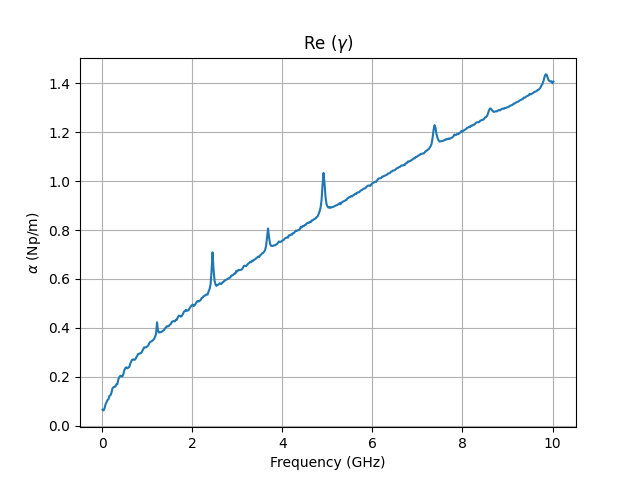
\includegraphics[width=\textwidth]{figures/gamma_real.png}
        \captionof{figure}{Componente real ($\alpha$) de la constante de propagación.}
        \label{fig:gamma_real}
        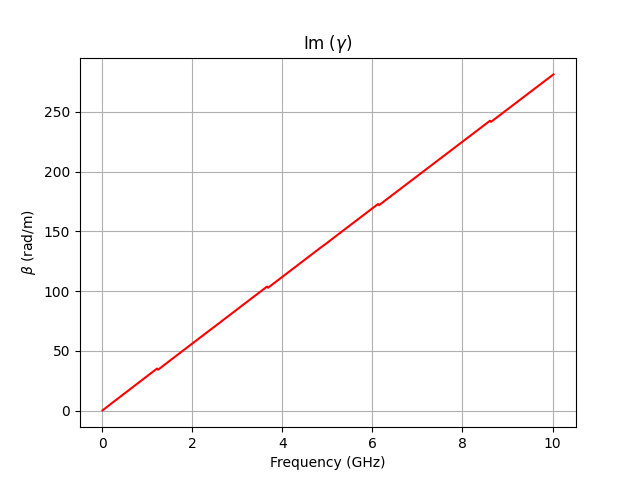
\includegraphics[width=\textwidth]{figures/gamma_imaginary.png}
        \captionof{figure}{Componente imaginaria ($\beta$) de la constante de propagación.}
        \label{fig:gamma_imag}

        {\centering\section*{\large Conclusiones}}
        El método matricial demostró ventajas como: Eliminar los saltos de fase en 90° y 180° mediante el criterio de continuidad (|B$_{m}$| > |$\frac{a_m}{c_m}$|)
        y la capacidad para manejar líneas con desacoplamiento severo ($|\Gamma| > 0.7$). La relación entre los valores propios y $\gamma$ permitió una interpretación 
        física directa: la magnitud de $\lambda$ determina la atenuación ($\alpha$) mientras que su fase codifica la constante de fase ($\beta$).
    \end{minipage}
        %\printbibliography  % Print bibliography
\end{document}